\documentclass[tikz,border=5pt]{standalone}
\usepackage{amsmath}
\usetikzlibrary{positioning,fit,arrows.meta}

\begin{document}
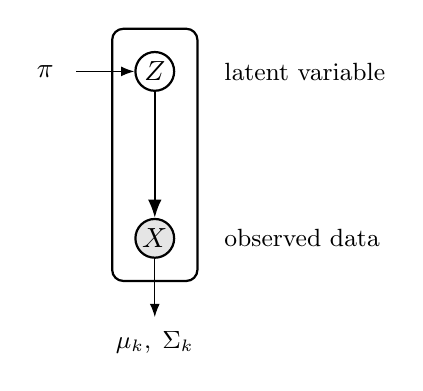
\begin{tikzpicture}[
    latent/.style={circle,draw,thick,minimum size=14pt,inner sep=0pt},
    observed/.style={latent,fill=gray!20},
    plate/.style={draw,thick,rounded corners,inner sep=8pt},
    >=Latex
]

% nodes
\node[latent]   (Z)          {$Z$};
\node[observed] (X) [below=1.6cm of Z] {$X$};

% arrow Z -> X
\draw[->,thick] (Z) -- (X);

% labels on the right
\node[right=0.5cm of Z] {\small latent variable};
\node[right=0.5cm of X] {\small observed data};

% prior / parameters
\draw[<-] (Z) --++ (-1,0);
\draw[->] (X) --++ (0,-1);
\node[left=0.9cm of Z]  {$\pi$};
\node[below=0.8cm of X] {\small $\mu_k,\;\Sigma_k$};

% plate surrounding the generative block
\node[plate,fit=(Z)(X)] (plate1) {};

\end{tikzpicture}
\end{document}